\documentclass[]{article}

\usepackage{mathtools,mathrsfs,url,fancyhdr, graphicx,amssymb,esvect}

\renewcommand{\headrulewidth}{0pt}
\fancyhead[L]{}
\fancyhead[C]{
	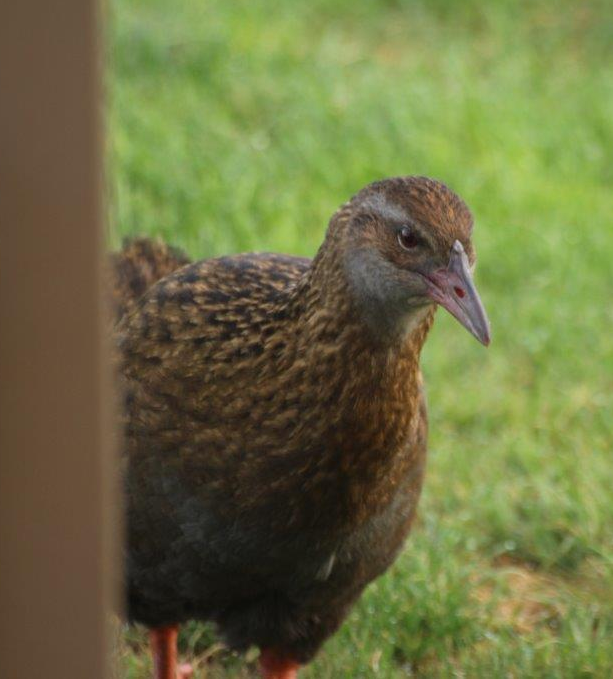
\includegraphics[width=2cm]{weka.png}
}

\newcommand\numberthis{\addtocounter{equation}{1}\tag{\theequation}}

\graphicspath{ {images/} }
\newcommand{\Lagr}{\mathscr{L}}
\pagestyle{plain}

%opening
\title{Introduction into General Relativity\\Assignment 3--Problem 1\\The stress--energy tensor $T^{\mu\nu}$ for the dust}
\author{Simon Crase}

\begin{document}

\maketitle
\thispagestyle{fancy}


\section{Variation of the Action}

For the dust, \cite[(90)]{akhmedev2016} gives the following.
\begin{align*}
S_M &= - \sum_{q=1}^N m_q \, \int d\tau_q \, \sqrt{g_{\mu\nu}[z_q(\tau_q)] \, \dot{z}_q^\mu(\tau_q)\, \dot{z}_q^\nu(\tau_q)}\\
&= - \int d^4 x \sum_{q=1}^N m_q \underbrace{\int d \tau_q \delta^{(4)} \big[x - z_q(\tau_q)\big]}_\text{As in \cite[(72)]{akhmedev2016}} \sqrt{g_{\mu\nu}[z_q(\tau_q)] \, \dot{z}_q^\mu(\tau_q)\, \dot{z}_q^\nu(\tau_q)} \\
&= - \int d^4 x \sum_{q=1}^N m_q \underbrace{\int d \tau \delta^{(4)} \big[x - z_q(\tau)\big] \sqrt{g_{\mu\nu}[z_q(\tau)] \, \dot{z}_q^\mu(\tau)\, \dot{z}_q^\nu(\tau)}}_\text{We can suppress the index on $\tau_q$ without confusion} \\
&\text{hence}\\
\delta_{g} S_M &= - \int d^4 x \sum_{q=1}^N m_q \int d \tau \delta^{(4)} \big[x - z_q(\tau)\big] \delta_{g} \big[\sqrt{g_{\mu\nu}[z_q(\tau)] \, \dot{z}_q^\mu(\tau)\, \dot{z}_q^\nu(\tau)}\big] \\
&= - \int d^4 x \sum_{q=1}^N m_q \int d \tau \delta^{(4)} \big[x - z_q(\tau)\big] \frac{ \dot{z}_q^\alpha(\tau) \dot{z}_q^\beta(\tau) \delta g_{\alpha\beta}}{2 \sqrt{g_{\mu\nu}[z_q(\tau)] \, \dot{z}_q^\mu(\tau)\, \dot{z}_q^\nu(\tau)}} \\
&= - \frac{1}{2} \int d^4 x \sum_{q=1}^N m_q \int d \tau \delta^{(4)} \big[x - z_q(\tau)\big] \frac{ \dot{z}_q^\alpha(\tau) \dot{z}_q^\beta(\tau) \delta g_{\alpha\beta}}{ \sqrt{g_{\mu\nu}[z_q(\tau)] \, \dot{z}_q^\mu(\tau)\, \dot{z}_q^\nu(\tau)}} \numberthis \label{eq:variation_of_action}
\end{align*}





\section{The Energy Momentum Tensor $T_{\mu\nu}$}

\begin{align}
T_{\mu\nu}&\triangleq 2 \frac{\partial \Lagr}{\partial g^{\mu\nu}} - \Lagr g_{\mu\nu} \label{eq:T}\\
&= -2 \frac{\partial }{\partial g^{\mu\nu}}\sum_{q=1}^N \sqrt{g^{\mu\nu}(z) p_{q,\mu} p_{q,\nu}}+\sum_{q=1}^N \sqrt{ p^{\sigma}_q p_{q,\sigma}} g_{\mu\nu} \\
&= - \sum_{q=1}^N \frac{2 p_{q,\mu} p_{q,\nu}}{2 \sqrt{ p^{\sigma}_q p_{q,\sigma}} }  +\sum_{q=1}^N \sqrt{ p^{\sigma}_q p_{q,\sigma}} g_{\mu\nu} \\
&= - \sum_{q=1}^N \frac{p_{q,\mu} p_{q,\nu}}{ m_{q,0} c }  +c\sum_{q=1}^N   m_{q,0} g_{\mu\nu} 
\end{align}
The last step follows from \cite{wiki_momentum}, where $m_q,0$ is the mass of the qth point in its co-moving frame. \emph{The minus sign looks dodgy!}


In the comoving frame of the $qth$ particle,
\begin{align}
\frac{p_{q,\mu} p_{q,\nu}}{ m_{q,0} c } =& \frac{m_{q,0}}{c}  u_{\mu}(z_q) u_{\nu}(z_q)\\
=& \frac{m_{q}}{\sqrt(|g|)}  u_{\mu}(z_q) u_{\nu}(z_q) \label{eq:PP}
\end{align}
Where $u_{\nu}(z)$ is the velocity field at a general position $z$, and $z_q$ is the position of the $qth$ particle. Now (\ref{eq:PP}) is a tensor equation, so we can use it in any frame to derive.
\begin{align}
T_{\mu\nu} &= - \sum_{q=1}^N  \frac{m_{q}}{\sqrt(|g|)}  u_{\mu}(z_q) u_{\nu}(z_q)  +c\sum_{q=1}^N   m_{q,0} g_{\mu\nu}\\
T^{\mu\nu} &= - \sum_{q=1}^N  \frac{m_{q}}{\sqrt(|g|)}  u^{\mu}(z_q) u^{\nu}(z_q)  +c\sum_{q=1}^N   m_{q,0} g^{\mu\nu}
\end{align}

From the lecture we know that:

$$\delta_g S_M = \frac{1}{2} \int d^4 x \sqrt{|g(x)|} T_{\mu\nu} \delta g^{\mu\nu}$$


Using the relation $\delta g_{\mu\nu} = − g_{\mu\alpha} \delta g ^{\alpha\beta} g_{\beta\nu}$, which was proved in the lecture, one can show that $T^{\mu\nu} \delta g_{\mu\nu} = - T_{\mu\nu} \delta g^{\mu\nu}$

Then for $T^{\alpha\beta}$ we have

\begin{align*}
T^{\alpha\beta} =& \frac{1}{\sqrt{|g(x)|}} \sum_{q=1}^{N} \int d\tau \delta^{(4)} \big[x-z_q(\tau)\big]\frac{\dot{z_q^\alpha} \dot{z_q^\beta}}{\sqrt{g_{\mu\nu}(z)\dot{z_q^\mu}\dot{z_q^\nu}}} \\
=& \frac{1}{\sqrt{|g(x)|}} \sum_{q=1}^{N} \int d\tau \delta^{(3)} \frac{\big[\vv{x}-\vv{z}_q(\tau)\big]}{\dot{z}_q^0}\frac{\dot{z_q^\alpha}  \dot{z_q^\beta}}{\sqrt{g_{\mu\nu}(z)\dot{z_q^\mu}\dot{z_q^\nu}}}
\end{align*}


where in the last line we have taken the $d\tau$ integral with the use of one of the $\delta-$ functions.

Using that $\sqrt{g_{\mu\nu}(z)\dot{z_q^\mu}\dot{z_q^\nu}}=s$, where s is the proper time, we arrive at:

$T^{\alpha\beta}(x) = \frac{1}{\sqrt{|g(x)|}} \sum_{q=1}^{N} \int d\tau \delta^{(3)} \frac{\big[\vv{x}-\vv{z}_q(s)\big]}{u_q^0 (s)} u_q^\alpha (s) u_q^\beta (s)$

Here now $u^{\mu} = \dot{z^\mu} = \frac{d z^\mu}{d s}$


\section{The Energy Density $\rho$}

\begin{align}
\rho(x) &= T^{\mu\nu}(x) \, u_\mu(x) \, u_\nu(x)
\end{align}


$\rho = \frac{1}{\sqrt{|g|}} \sum_{q=1}^{N} m_q \frac{d z^0_q}{d s} \delta^{(3)} \big[\vv{x}-\vv{z}_q(s)\big]$ 

$\frac{d z^0_q}{d s}=\gamma$

\begin{thebibliography}{9}
	
	\bibitem{akhmedev2016}
	Emil T. Akhmedev,
	\emph{Lectures on General Theory of Relativity},
	2016,
	\url{https://arxiv.org/pdf/1601.04996v6.pdf}.
	
	\bibitem{wiki_delta}
	Wikipedia,
	\emph{The Dirac Delta Function}
	\url{https://en.wikipedia.org/wiki/Dirac_delta_function#Composition_with_a_function},
	Retrieved: 19 February 2017
	
	\bibitem{wiki_momentum}
	Wikipedia,
	\emph{Energy Momentum Relation}
	\url{https://en.wikipedia.org/wiki/Energy%E2%80%93momentum_relation#General_relativity}
		Retrieved: 19 February 2017
\end{thebibliography}

\end{document}
